\subsection{Technical Overview}
	The following requirements need to be supported by the technologies chosen to implement CPP 2.0:
		\begin{itemize}
		  \item \textbf{User Interface:} Produce an innovative user experience providing a responsive profile based experience that encapsulates the user and makes the system enjoyable and intuitive to use. This results in the need for a fast client side interaction with a professional user interface.
		  \item \textbf{Database:} User, Company and Admin information needs to be stored in an organised and easily accessible format.
		  \item \textbf{Security:} Handling student private data such as their CVs is sensitive information, we need a way to securely store such information 
		\end{itemize} 

	\subsubsection{Server-Side Overview}
		CPP 2.0: Connected uses:
		\paragraph{Ruby on Rails (Rails)\cite{ror}} as a web framework for storing persistent data and communicating it to the front-end of the system. Rails uses a Model View Controller design pattern to organise the back-end structure, providing secure and efficient storage of persistent user information. The following schema entity relationship diagram details the setup of the different entities within the back-end Rails server.
		%\begin{center}
		    %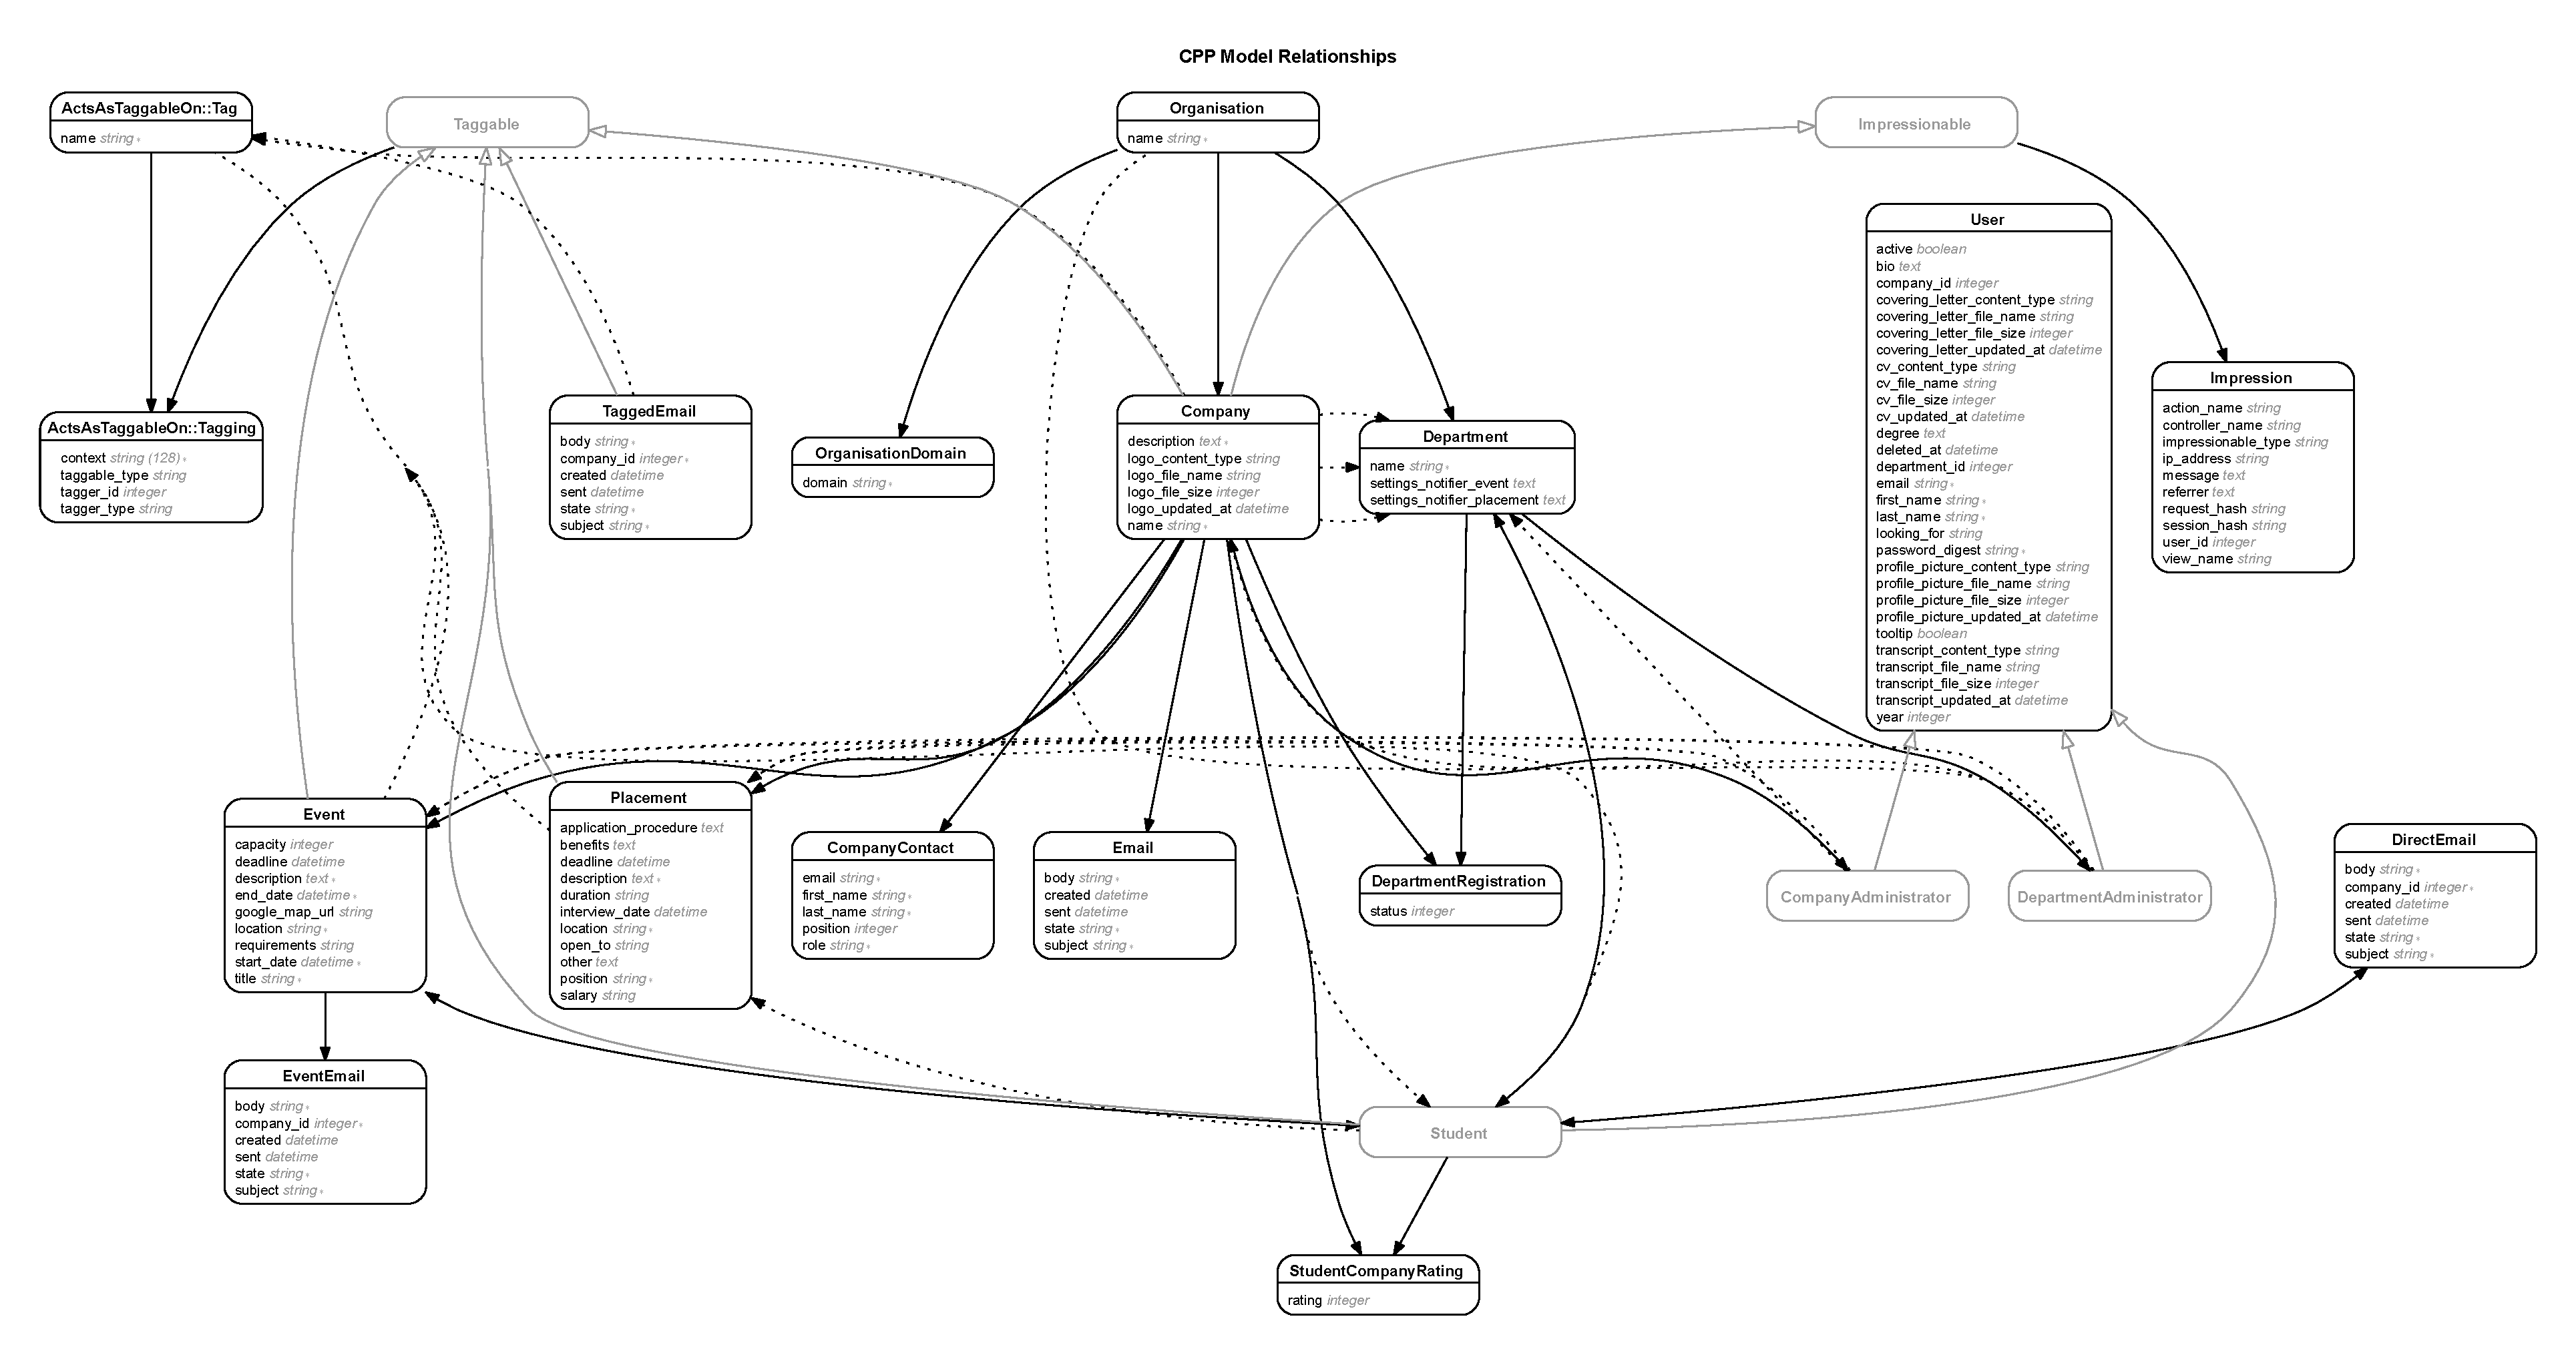
\includegraphics[scale=0.3]{images/implementation/technical_overview/erd}
		%\end{center}
		%TODO: I'm just trying to write about how it's got a really nice DB
		Rails helps us to meet our technological requirements by using a Model View Controller architecture pattern where by each model maps to a table in a database, a controller responds to external requests from the web server, and we have chosen to implement JavaScript views rather than Rails views.
		Very usefully Rails allows us to avoid using raw SQL to find database records and provides a vast amount of methods for extracting data from a table. We feel this approach is much more clear and intuative to a programmer and has overall been less error prone than if we would have had to write our own queries. %TODO: Perhaps appendicise some of the really useful ones 

		Rails provides an elegant and succinct way to communicate with the front-end implemented in Backbone and supports all features that our project requires. 

		\paragraph{Ruby Gems\cite{gems}} are packaged Ruby applications or libraries and are another advantage of writing our project with Rails. There is a huge gem community and often someone has written a gem to provide the exact functionality we desire for something. This saves us time in implementing a large amount of code to acheive the feature we want and allows us to spend more time tiying this feature into our site. [TODO: Im not that keen on the phrasing of this, but it's what I want to say]. In our project we have made use of many gems such as
		\begin{itemize}
		 \item Paperclip\cite{paperclip} for easy file attachments with AWS S3\cite{s3} integration.
		 \item CanTango\cite{cantango} for restricting what resources students, departments and admins can access.
		 \item ActsAsTaggableOn\cite{tags} for seemless tag integration.
		\end{itemize}
	\subsubsection{Client-Side Overview}
		CPP 2.0: Connected uses:
		\paragraph{Backbone\cite{backbone}} to provide a highly interactive and responsive client-side experience. The Backbone library is essentially broken down into Models, Collections and Views that connect to the Rails server API using a RESTful JSON interface. Models contain the attributes of the data entities as well as the logic surrounding them, Collections are ordered sets of models with a rich API of enumerable functions and Views concern the presentation logic with declarative event handling. Backbone implements a Model View Controller (MVC) design pattern which applies the ‘separation of  concerns’ principle, this results in improved structure and organization of code.
		\paragraph{CoffeeScript\cite{coffeescript}} is used as an alternative to Javascript due to its layer of beautiful syntactic sugar that allows us to produce Javascript in a really succinct and efficient way. This results in more efficient, neater code as well as longterm increased code production speed.
		\paragraph{Twitter Bootstrap\cite{bootstrap}} is a front-end framework used to present a clean and simple user interface that supports dynamic scaling to different screen sizes. We chose Bootstrap for this reason and because it provides many useful JavaScript plugins such as the typeahead for our student degree and tag input fields. It provides nice visuals with very little setup which was perfect for our timeframe of this project. We would not have had time to have designed the CSS ourselves.